%% Dokumenteinstellungen %%%%%%%%%%%%%%%%%%%%%%%%%%%%%%%%%%%%
\documentclass[a4paper,oneside,12pt,ngerman]{scrartcl}

%% Deutsche Anpassungen %%%%%%%%%%%%%%%%%%%%%%%%%%%%%%%%%%%%%
\usepackage[ngerman]{babel}
\usepackage[T1]{fontenc}
\usepackage[ansinew]{inputenc}
\usepackage{lmodern} %Type1-Schriftart f�r nicht-englische Texte
\usepackage{booktabs}	% sch�nere tabellen

%% Packages f�r Grafiken & Abbildungen %%%%%%%%%%%%%%%%%%%%%%
\usepackage{graphicx} %%Zum Laden von Grafiken
%\usepackage{subfig} %%Teilabbildungen in einer Abbildung
%\usepackage{tikz} %%Vektorgrafiken aus LaTeX heraus erstellen


%% Packages f�r Formeln %%%%%%%%%%%%%%%%%%%%%%%%%%%%%%%%%%%%%
\usepackage{amsmath}
\usepackage{amsthm}
\usepackage{amsfonts}


%% Andere Packages %%%%%%%%%%%%%%%%%%%%%%%%%%%%%%%%%%%%%%%%%%
%\usepackage{a4wide} %%Kleinere Seitenr�nder = mehr Text pro Zeile.
\usepackage{fancyhdr} %%Fancy Kopf- und Fu�zeilen
%\usepackage{longtable} %%F�r Tabellen, die eine Seite �berschreiten
\usepackage{lastpage}
\usepackage[raggedright]{subfigure}
\usepackage[final]{pdfpages}
\includepdfset{pages=-,noautoscale}

%%%%%%%%%%%%%%%%%%%%%%%%%%%%%%%%%%%%%%%%%%%%%%%%%%%%%%%%%%%%%
%% TODO
%%%%%%%%%%%%%%%%%%%%%%%%%%%%%%%%%%%%%%%%%%%%%%%%%%%%%%%%%%%%%
% 
% 
%%%%%%%%%%%%%%%%%%%%%%%%%%%%%%%%%%%%%%%%%%%%%%%%%%%%%%%%%%%%%



%%%%%%%%%%%%%%%%%%%%%%%%%%%%%%%%%%%%%%%%%%%%%%%%%%%%%%%%%%%%%
%% Optionen / Modifikationen
%%%%%%%%%%%%%%%%%%%%%%%%%%%%%%%%%%%%%%%%%%%%%%%%%%%%%%%%%%%%%
%%%%%%%%%%%%%%%%%%%%%%%%%%%%%%%%%%%%%%%%%%%%%%%%%%%%%%%%%%%%%
%%                                                         %%
%%                     EINSTELLUNGEN                       %%
%%                                                         %%
%%%%%%%%%%%%%%%%%%%%%%%%%%%%%%%%%%%%%%%%%%%%%%%%%%%%%%%%%%%%%

%%%%%%%%%%%%%%%%%%%%%%%%%%%%%%%%%%%%%%%%%%%%%%%%%%%%%%%%%%%%%
%% HYPER REF
%%%%%%%%%%%%%%%%%%%%%%%%%%%%%%%%%%%%%%%%%%%%%%%%%%%%%%%%%%%%%
\usepackage[
hyperindex=true,
colorlinks=true,
linkcolor=black,
citecolor=black,
filecolor=black,
menucolor=black,
urlcolor=cyan,
breaklinks=true,
bookmarks=true,
bookmarksopen=false,
bookmarksnumbered=false,
pdfhighlight=/O,
]{hyperref}

%%%%%%%%%%%%%%%%%%%%%%%%%%%%%%%%%%%%%%%%%%%%%%%%%%%%%%%%%%%%%
%% FANCY HEADERS
%%%%%%%%%%%%%%%%%%%%%%%%%%%%%%%%%%%%%%%%%%%%%%%%%%%%%%%%%%%%%
% --- Kopf- und Fusszeilen - {} = rechts (gerade), [] = links (ungerade)
% letzte seite: \pageref{LastPage}
% doppelseitig:
%\lhead{Elektronik: \textbf{Oszilatorschaltungen}}	\chead{}		\rhead{Cyril Stoller und Hannes Stauffer}
%\lfoot{\today}	\cfoot{}		\rfoot{Seite \thepage\ von \pageref{LastPage}}

% einseitig:
%\lhead{\rightmark}			\chead{}					\rhead{}
%\lfoot{\leftmark}			\cfoot{}					\rfoot{Seite \thepage\ von \pageref{\LastPage}}

%\setlength{\headrulewidth}{0.4pt}
%\setlength{\footrulewidth}{0.4pt}


% Formeln r�misch nummerieren
\renewcommand{\theequation}{\Roman{equation}} 

% "Formel" statt "Gleichung"
\def\equationname{Formel}

%%%%%%%%%%%%%%%%%%%%%%%%%%%%%%%%%%%%%%%%%%%%%%%%%%%%%%%%%%%%%
%% DOKUMENT
%%%%%%%%%%%%%%%%%%%%%%%%%%%%%%%%%%%%%%%%%%%%%%%%%%%%%%%%%%%%%
\begin{document}

\title{Projektarbeit: Buckconverter (Step-Down)}
\date{\today}
\author{Cyril Stoller, Jascha Haldemann, Marcel B�rtschi, Nicola K�ser}
\maketitle


%\pagestyle{fancy} %%Ab hier die Kopf-/Fusszeilen: headings / fancy / ...

\vspace{1cm}


%%%%%%%%%%%%%%%%%%%%%%%%%%%%%%%%%%%%%%%%%%%%%%%%%%%%%%%%%%%%%
%%                                                         %%
%%         Kapitel / Hauptteil des Dokumentes              %%
%%                                                         %%
%%%%%%%%%%%%%%%%%%%%%%%%%%%%%%%%%%%%%%%%%%%%%%%%%%%%%%%%%%%%%

\section{Ziel/Einleitung}
Anhand eines Stepdown (Buck) Converters soll die erarbeitete Theorie �ber Leistungselektronik angewendet werden. Die Diode und der MOSFET sind vorgegeben und die Drossel und der Kondensator m�ssen dimmensioniert werden.
Mithilfe der Theorie und der Application Note von Infineon sollen alle Berechnungen f�r die Verluste durchgef�hrt werden. Alle Werte sollen f�r einen Eingangsspannungsbereich von 12-75 Volt, eine Ausgangsspannung von 10-30 Volt und einen Ausgangsstrom von 1-10 Amp�re berechnet werden. 

Dieser Bericht erl�utert die Funktionsweise des Buckconverters, zeitg die Berechnung und die Auswertung der Wirkungsgrade und noch die Dimmensionierung der passiven Komponenten (Drossel und Kondensator). Die Funktionsweise des Regel-IC's (PWM-Generator) wird weggelassen.

Alle Berechnungen wurden in einem Matlab Skript (Buckconverter.m) durchgef�hrt, welches diesem Bericht beiliegt. Auf die genaue implementierung wird in diesem Bericht nicht eingegangen. Es wird vorausgesetzt, dass ein grundlegendes Verst�ndnis der Matlab Skriptsprache vorhanden ist. Somit ist der Code (mit dem Komentar) selbsterkl�rend.

\section{Schema}
Ein Buckconverter oder Abw�rtswandler funktioniert nach folgendem Schema. Die PWM-Ansteuerung des MOSFET wurde hier einfachhietshalber weggelassen. Zudem nehmen wir an, dass der Wandler immer im kontinuierlichen Betrieb arbeitet. Das heisst, der Strom am Ausgang $I_0$ wird nie null. Somit wird in der On-Phase (MOSFET leitet) der Strom durch die Spule nach dem Induktionsgesetz ansteigen. Schaltet nun der MOSFET ab, liegt �ber der Spule im wesentlichen die Ausgangsspannung, wodurch damach der Strom $I_L$ linear abf�llt. Damit ergibt sich am Ausgang gemittelt �ber die Zeit eine konstante Spannung $U_0$, welche mit dem Kondensator noch etwas gegl�ttet wird.

\begin{figure}[ht]
	\centering
		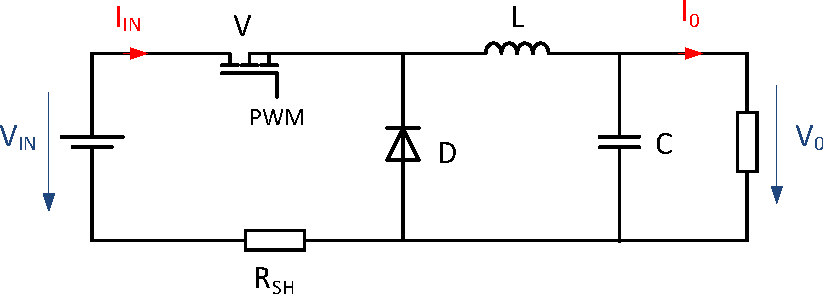
\includegraphics[width=0.90\textwidth]{pics/schema.pdf}
	\caption{Schema Stepdown Converter}
	\label{fig:schema}
\end{figure}

\section{Duty Cycle}
Um den Duty Cycle zu bestimmen sind wir nach Fomel \ref{formel:DutyCycle} vorgegangen. Im Matlabsktipt haben wir f�r alle Werte, welche in einem gewissen Bereich variieren Matrizen erstellt. Somit k�nnen wir einfach elementweise alle Werte berechnen, ohne mit Loops zu arbeiten. Dies ist viel anschaulicher und intuitiv lesbar. 

\begin{align}
	\label{formel:DutyCycle}
		D =\frac{(V_0 + (R_l + R_0) \cdot I_0 + V_{f0})}{(V_{in} - (R_{DSon} + R_{sh} - R_0) \cdot I_0 + V_{f0})} 
\end{align}

Aus dieser Formel ergibt sich f�r die Ein- bzw. Ausgangsspannung bei 10 Ampere folgende Grafik:

\begin{figure}[ht]
	\centering
		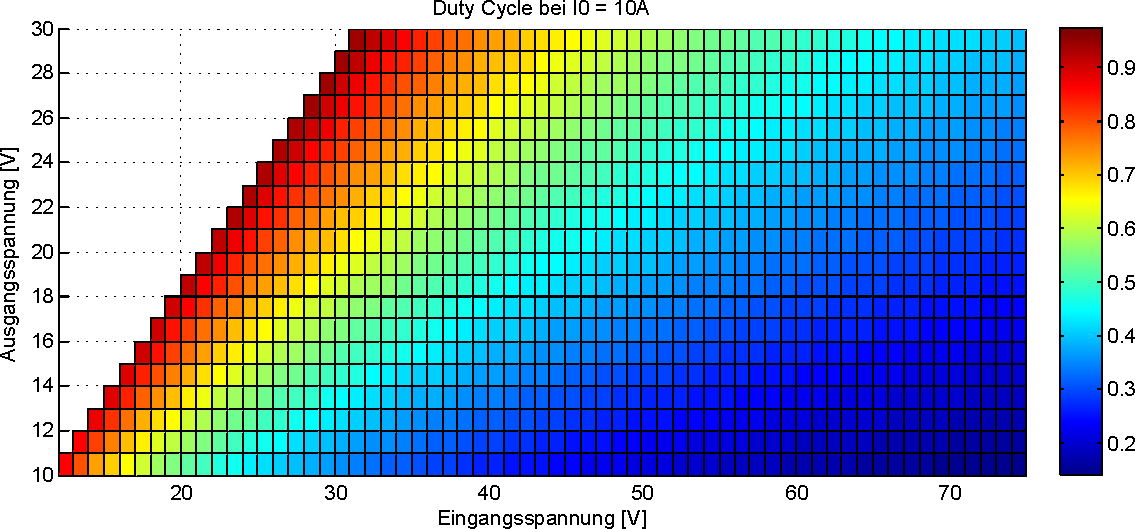
\includegraphics[width=1\textwidth]{pics/DutyCycle.pdf}
	\caption{Duty Cycle bei 10A}
	\label{fig:Duty Cycle}
\end{figure}
Man erkennt gut, dass dort wo die Ausgangsspannung praktisch gleichgross ist wie die Eingangsspannung der Duty Cycle beinahe eins wird. Dies macht ja auch Sinn, denn in diesem Fall muss beinahe die gesamte Eingangsleistung an den Ausgang weitergegeben werden. 

\section{Wirkungsgrad}
Um den Wirkungsgrad zu bestimmen muss zuerst die gesamte Verlustleistung ausgerechnet werden. Dies enth�lt die Schalt-und Leitverluste. Die Leckverluste werden vernachl�ssigt. 
\subsection{Leitverluste}
Die Leitverluste werden mit einfachen Modellen der Bauteile berechnet. Dabei wird z.B. beim MOSFET nur der Drain-Source Widerstand bestimmt und mit dem Quadrat des Effektivwerts des durchfliessenden Stromes multipliziert. 

\subsection{Schaltverluste}
Diese Berechnung war wohl der aufw�ndigste Teil unseres Projekts. Um die Schaltverluste zu berechnen m�ssen einige Werte aus Datenbl�ttern ausgelesen werden und danach richtig in die Formel eingesetzt werden. 

Erstaundlich ist, dass die Schaltverluste (bei $I_0$ fix) linear zur Ausgangsspannung und total unabh�ngig von der Eingangsspanung sind. Ebenso erstaundlich ist die Tatsache dass es sich bei den Schaltverlusten um recht grosse Leistungen ($P_{Smax} = 1.105W$) handelt.
\subsection{Auswertung Wirkungsgrad}
Berechnen wir nun den Wirkungsgrad ergibt sich f�r $I_0$ folgendes Bild:

\begin{figure}[ht]
	\centering
		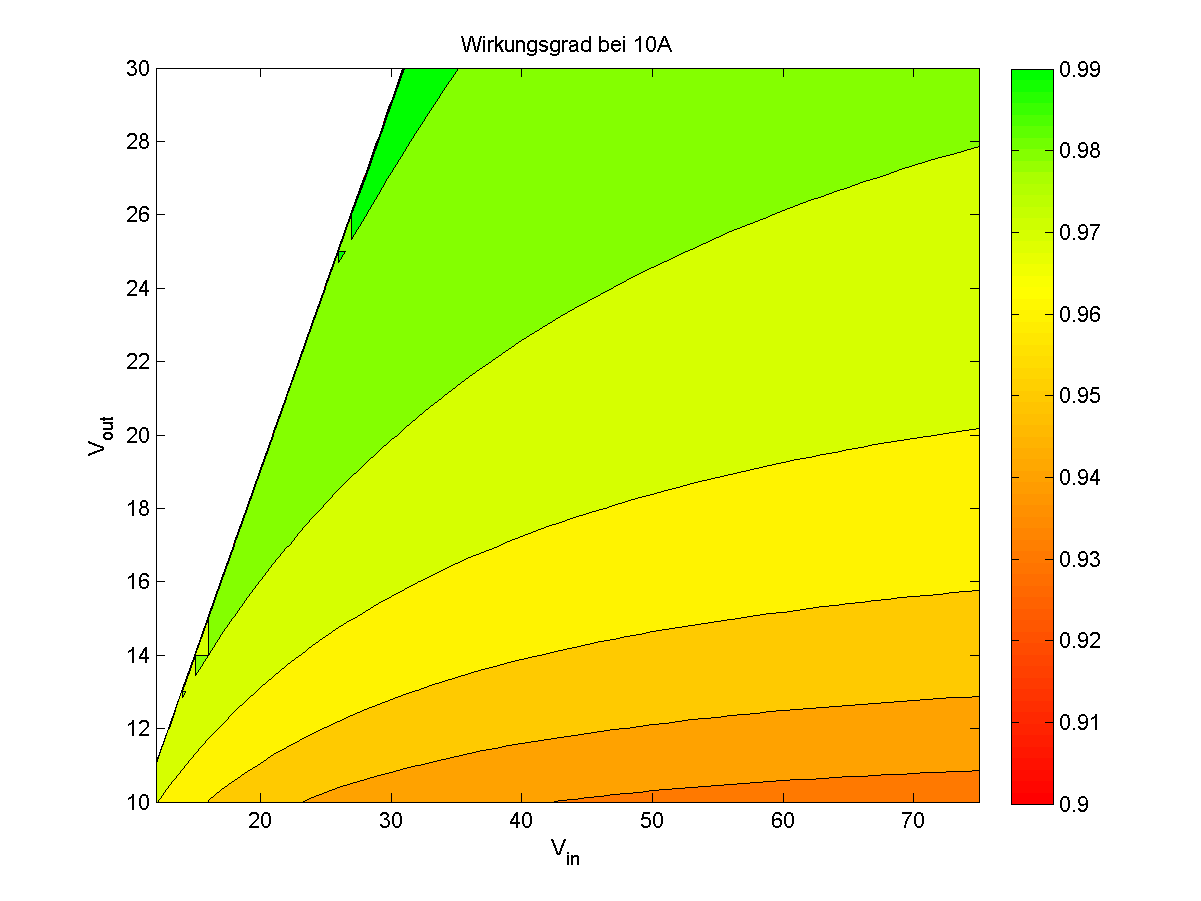
\includegraphics[width=0.61\textwidth]{pics/grafik_10A.png}
	\caption{Wirkungsgrad bei 10A}
	\label{fig:Wirkungsgrad}
\end{figure}

Das Matlabskript erstellt automatisch Bilder des Wirkungsgrades f�r 1..10A und speichert diese im Ordner \textit{pics}.

Man erkannt hier einen Worst-Case Wirkungsgrad bei $V_{IN}$, $V_0$ und $I_0$ von etwa 93\%. Dieses Resultat erscheint realistisch und ist etwa in der Gr�ssenordnung wo wir es haben m�chten. 

\section{Dimensionierung Drossel}
Die Spule kann berechnet werden, indem man beim maximalen Rippel $\Delta$i (20\% von $I_{0max}$ gew�hlt) die Spannung �ber der Spule bestimmt. 
\begin{align}
	\label{formel:b}
	U_L=L\cdot\frac{di}{dt} 
\end{align}
Die Formel \ref{formel:b} kann f�r kleine $\Delta$i und kurze Zeiten folgendermassen approximiert werden:
\begin{align}
	U_L=L\cdot\frac{\Delta i}{D\cdot T} 
\end{align}
Wobei D der Duty Cycle und T die Periodendauer sind.
Stellt man die Gleichung nach L um und berechnet die Spannung $U_L$ nach Kirchhofschem Maschensatz, eh�lt man die Gleichung:
\begin{align}
	\begin{split}
		L &= \frac{(V_{IN}-V_{0}-(R_{SH}+R_{DSon})\cdot I_0)\cdot D \cdot T}{\Delta i} \\
		&=\frac{(75V-30V-(10m\Omega+2.7m\Omega)\cdot 10A)\cdot 0.4074 \cdot 12.5\mu s}{2A} = 114\mu H
	\end{split}
\end{align}



\subsection{Rippel des Stromes $\Delta$i}

\begin{figure}[ht]
	\centering
		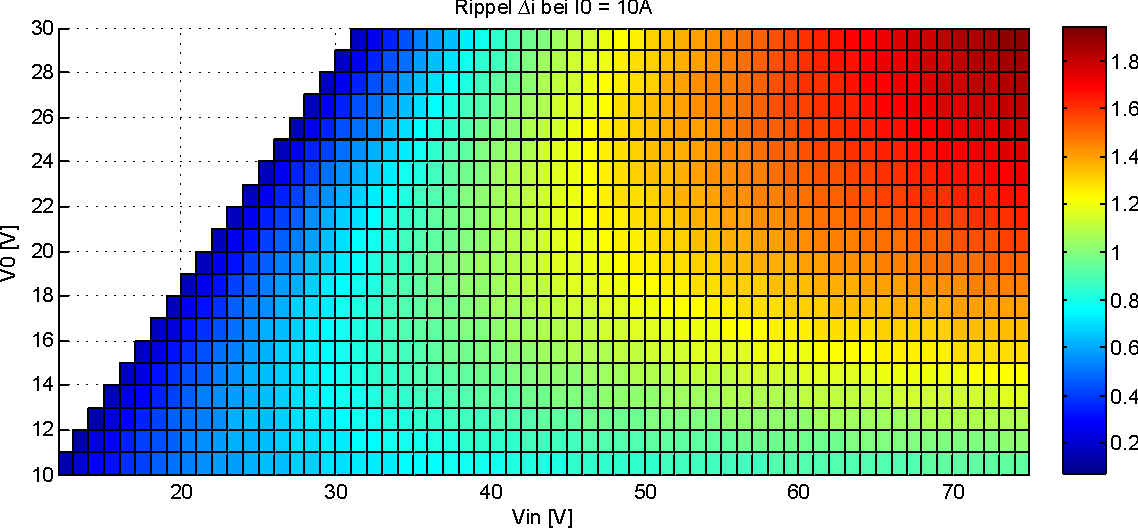
\includegraphics[width=1\textwidth]{pics/Rippel10A_3.pdf}
	\caption{Rippel bei 10A}
	\label{fig:Rippel}
\end{figure}

\section{Dimensionierung Kondensator}

%% Der Anhang kommt auf eine neue Zeile
%\newpage
%% Offizielle "A Anhang" Aufz�hlungsvariante
%\appendix
%% Nur im Inhaltsverzeichnis hinzuf�gen (mit richtiger Seite, da vorher "\newpage"), aber kein Text
%\addcontentsline{toc}{section}{Anhang}
%
%% Quellenverzeichnis
%%\addcontentsline{toc}{section}{Quellenverzeichnis}
%\section{Quellenverzeichnis}
%\renewcommand\refname{}
%
%\vspace{-1cm}
%
%\bibliographystyle{amsplain}
%\bibliography{Bildquellen}

\end{document}
